\section{oosalizer/hashtab.c-Dateireferenz}
\label{hashtab_8c}\index{oosalizer/hashtab.c@{oosalizer/hashtab.c}}
{\tt \#include $<$time.h$>$}\par
{\tt \#include $<$stdio.h$>$}\par
{\tt \#include $<$stdlib.h$>$}\par
{\tt \#include $<$string.h$>$}\par
{\tt \#include $<$unistd.h$>$}\par
{\tt \#include $<$ctype.h$>$}\par
{\tt \#include $<$sys/utsname.h$>$}\par
{\tt \#include $<$sys/times.h$>$}\par
{\tt \#include $<$sys/types.h$>$}\par
{\tt \#include \char`\"{}webalizer.h\char`\"{}}\par
{\tt \#include \char`\"{}lang.h\char`\"{}}\par
{\tt \#include \char`\"{}linklist.h\char`\"{}}\par
{\tt \#include \char`\"{}hashtab.h\char`\"{}}\par


Include-Abh\"{a}ngigkeitsdiagramm f\"{u}r hashtab.c:\begin{figure}[H]
\begin{center}
\leavevmode
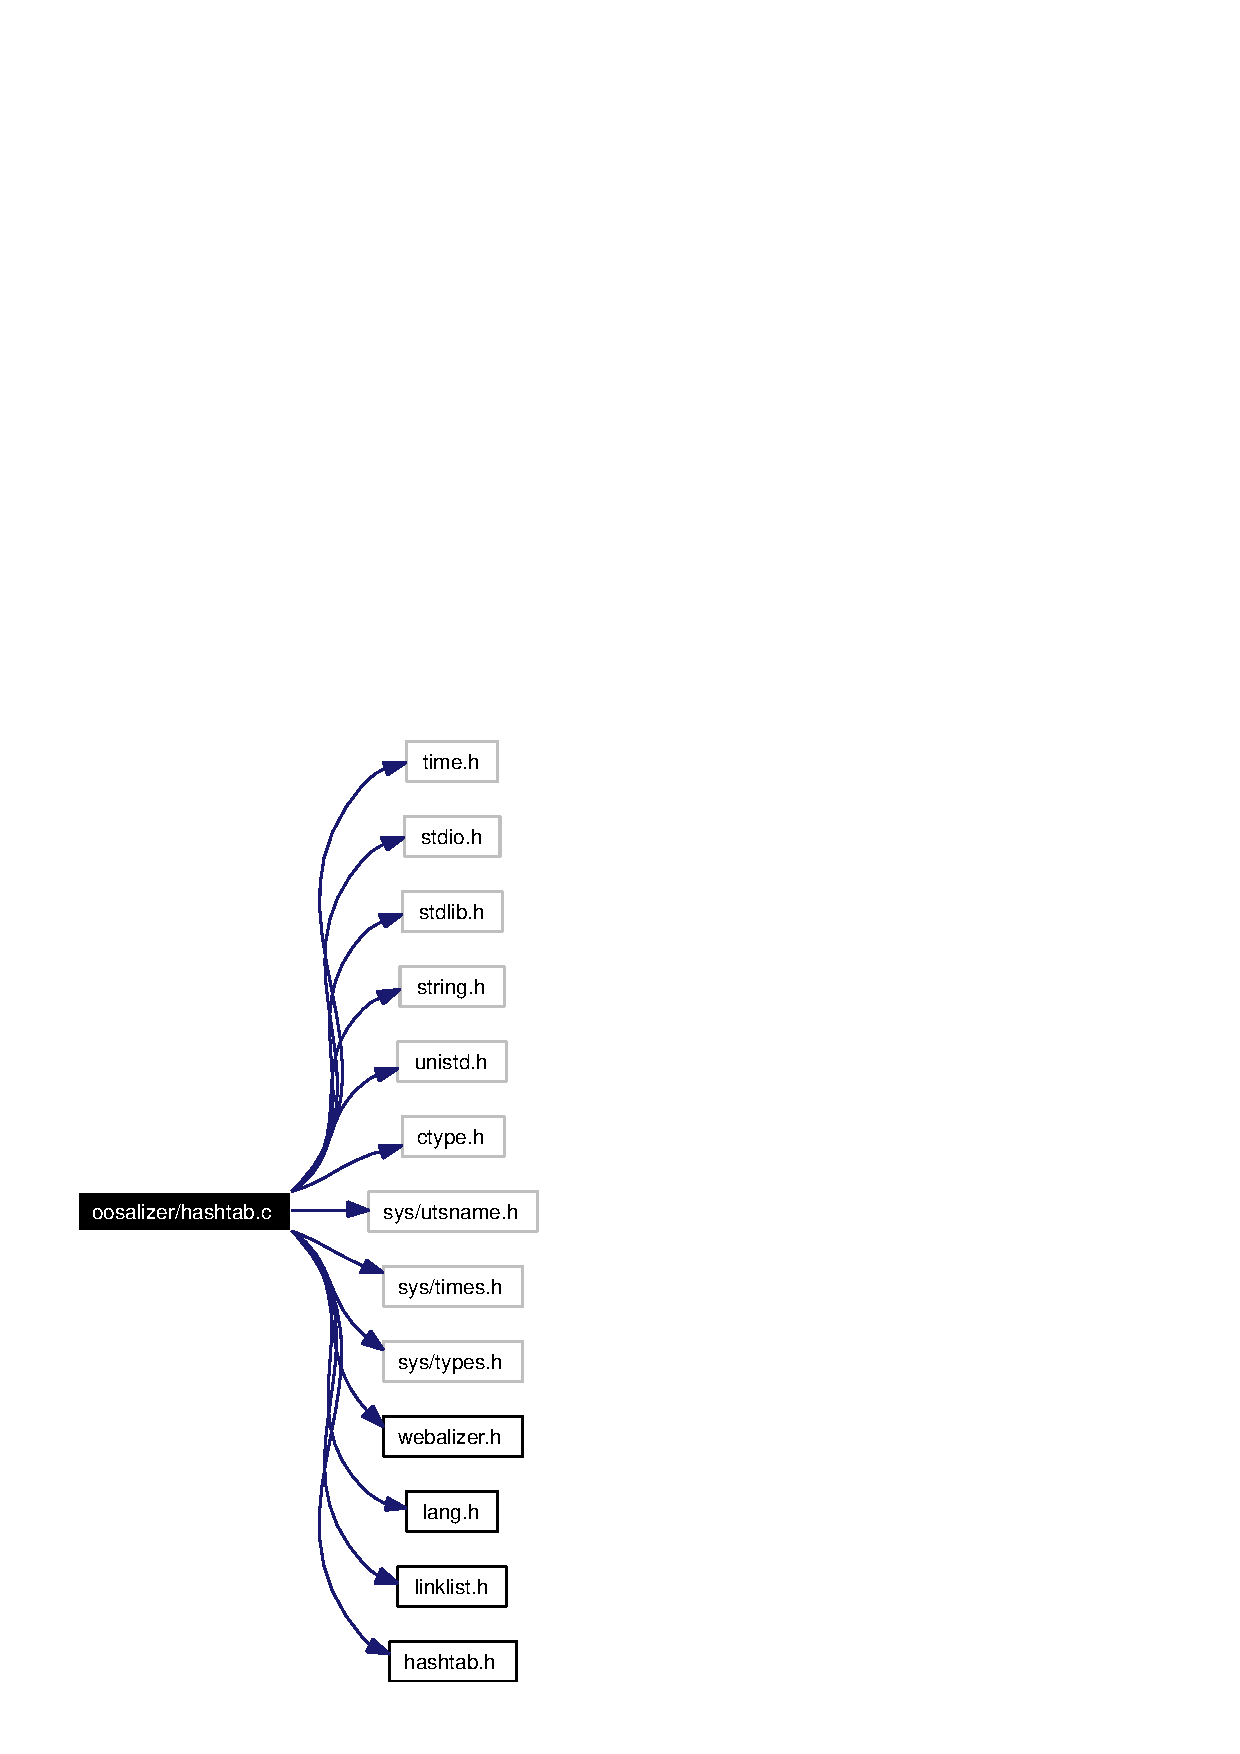
\includegraphics[width=129pt]{hashtab_8c__incl}
\end{center}
\end{figure}
\subsection*{Makrodefinitionen}
\begin{CompactItemize}
\item 
\#define {\bf CLK\_\-TCK}~\_\-SC\_\-CLK\_\-TCK
\end{CompactItemize}
\subsection*{Funktionen}
\begin{CompactItemize}
\item 
{\bf HNODEPTR} {\bf new\_\-hnode} (char $\ast$)
\item 
{\bf UNODEPTR} {\bf new\_\-unode} (char $\ast$)
\item 
{\bf RNODEPTR} {\bf new\_\-rnode} (char $\ast$)
\item 
{\bf ANODEPTR} {\bf new\_\-anode} (char $\ast$)
\item 
{\bf SNODEPTR} {\bf new\_\-snode} (char $\ast$)
\item 
{\bf INODEPTR} {\bf new\_\-inode} (char $\ast$)
\item 
void {\bf update\_\-entry} (char $\ast$)
\item 
void {\bf update\_\-exit} (char $\ast$)
\item 
u\_\-long {\bf hash} (char $\ast$)
\item 
void {\bf del\_\-htabs} ()
\item 
int {\bf put\_\-hnode} (char $\ast$str, int type, u\_\-long count, u\_\-long file, double xfer, u\_\-long $\ast$ctr, u\_\-long visit, u\_\-long tstamp, char $\ast$lasturl, {\bf HNODEPTR} $\ast$htab)
\item 
void {\bf del\_\-hlist} ({\bf HNODEPTR} $\ast$htab)
\item 
int {\bf put\_\-unode} (char $\ast$str, int type, u\_\-long count, double xfer, u\_\-long $\ast$ctr, u\_\-long entry, u\_\-long exit, {\bf UNODEPTR} $\ast$htab)
\item 
void {\bf del\_\-ulist} ({\bf UNODEPTR} $\ast$htab)
\item 
int {\bf put\_\-rnode} (char $\ast$str, int type, u\_\-long count, u\_\-long $\ast$ctr, {\bf RNODEPTR} $\ast$htab)
\item 
void {\bf del\_\-rlist} ({\bf RNODEPTR} $\ast$htab)
\item 
int {\bf put\_\-anode} (char $\ast$str, int type, u\_\-long count, u\_\-long $\ast$ctr, {\bf ANODEPTR} $\ast$htab)
\item 
void {\bf del\_\-alist} ({\bf ANODEPTR} $\ast$htab)
\item 
int {\bf put\_\-snode} (char $\ast$str, u\_\-long count, {\bf SNODEPTR} $\ast$htab)
\item 
void {\bf del\_\-slist} ({\bf SNODEPTR} $\ast$htab)
\item 
int {\bf put\_\-inode} (char $\ast$str, int type, u\_\-long count, u\_\-long file, double xfer, u\_\-long $\ast$ctr, u\_\-long visit, u\_\-long tstamp, {\bf INODEPTR} $\ast$htab)
\item 
void {\bf del\_\-ilist} ({\bf INODEPTR} $\ast$htab)
\item 
char $\ast$ {\bf find\_\-url} (char $\ast$str)
\item 
void {\bf month\_\-update\_\-exit} (u\_\-long tstamp)
\item 
u\_\-long {\bf tot\_\-visit} ({\bf HNODEPTR} $\ast$list)
\end{CompactItemize}
\subsection*{Variablen}
\begin{CompactItemize}
\item 
{\bf HNODEPTR} {\bf sm\_\-htab} [MAXHASH]
\item 
{\bf HNODEPTR} {\bf sd\_\-htab} [MAXHASH]
\item 
{\bf UNODEPTR} {\bf um\_\-htab} [MAXHASH]
\item 
{\bf RNODEPTR} {\bf rm\_\-htab} [MAXHASH]
\item 
{\bf ANODEPTR} {\bf am\_\-htab} [MAXHASH]
\item 
{\bf SNODEPTR} {\bf sr\_\-htab} [MAXHASH]
\item 
{\bf INODEPTR} {\bf im\_\-htab} [MAXHASH]
\end{CompactItemize}


\subsection{Makro-Dokumentation}
\index{hashtab.c@{hashtab.c}!CLK_TCK@{CLK\_\-TCK}}
\index{CLK_TCK@{CLK\_\-TCK}!hashtab.c@{hashtab.c}}
\subsubsection{\setlength{\rightskip}{0pt plus 5cm}\#define CLK\_\-TCK~\_\-SC\_\-CLK\_\-TCK}\label{hashtab_8c_03df76d1f70664d745ca8de2864e39b3}




Definiert in Zeile 59 der Datei hashtab.c.

\subsection{Dokumentation der Funktionen}
\index{hashtab.c@{hashtab.c}!del_alist@{del\_\-alist}}
\index{del_alist@{del\_\-alist}!hashtab.c@{hashtab.c}}
\subsubsection{\setlength{\rightskip}{0pt plus 5cm}void del\_\-alist ({\bf ANODEPTR} $\ast$ {\em htab})}\label{hashtab_8c_ebb84eee637f50db17ab93d1050e8bd1}




Definiert in Zeile 645 der Datei hashtab.c.

Benutzt MAXHASH, anode::next und anode::string.

Wird benutzt von del\_\-htabs().\index{hashtab.c@{hashtab.c}!del_hlist@{del\_\-hlist}}
\index{del_hlist@{del\_\-hlist}!hashtab.c@{hashtab.c}}
\subsubsection{\setlength{\rightskip}{0pt plus 5cm}void del\_\-hlist ({\bf HNODEPTR} $\ast$ {\em htab})}\label{hashtab_8c_306d5a1540d43fa136c10272cb2f0a4a}




Definiert in Zeile 283 der Datei hashtab.c.

Benutzt MAXHASH, hnode::next und hnode::string.

Wird benutzt von del\_\-htabs().\index{hashtab.c@{hashtab.c}!del_htabs@{del\_\-htabs}}
\index{del_htabs@{del\_\-htabs}!hashtab.c@{hashtab.c}}
\subsubsection{\setlength{\rightskip}{0pt plus 5cm}void del\_\-htabs ()}\label{hashtab_8c_f9fcdad76e91434fe5f0728f3a79ae74}




Definiert in Zeile 102 der Datei hashtab.c.

Benutzt am\_\-htab, del\_\-alist(), del\_\-hlist(), del\_\-ilist(), del\_\-rlist(), del\_\-slist(), del\_\-ulist(), im\_\-htab, rm\_\-htab, sd\_\-htab, sm\_\-htab, sr\_\-htab und um\_\-htab.

Wird benutzt von clear\_\-month().\index{hashtab.c@{hashtab.c}!del_ilist@{del\_\-ilist}}
\index{del_ilist@{del\_\-ilist}!hashtab.c@{hashtab.c}}
\subsubsection{\setlength{\rightskip}{0pt plus 5cm}void del\_\-ilist ({\bf INODEPTR} $\ast$ {\em htab})}\label{hashtab_8c_d859897805bb7fc6479703fd3bcf493a}




Definiert in Zeile 918 der Datei hashtab.c.

Benutzt MAXHASH, inode::next und inode::string.

Wird benutzt von del\_\-htabs().\index{hashtab.c@{hashtab.c}!del_rlist@{del\_\-rlist}}
\index{del_rlist@{del\_\-rlist}!hashtab.c@{hashtab.c}}
\subsubsection{\setlength{\rightskip}{0pt plus 5cm}void del\_\-rlist ({\bf RNODEPTR} $\ast$ {\em htab})}\label{hashtab_8c_99589c545676162533a82708505580c6}




Definiert in Zeile 529 der Datei hashtab.c.

Benutzt MAXHASH, rnode::next und rnode::string.

Wird benutzt von del\_\-htabs().\index{hashtab.c@{hashtab.c}!del_slist@{del\_\-slist}}
\index{del_slist@{del\_\-slist}!hashtab.c@{hashtab.c}}
\subsubsection{\setlength{\rightskip}{0pt plus 5cm}void del\_\-slist ({\bf SNODEPTR} $\ast$ {\em htab})}\label{hashtab_8c_d526188ebf65c97a2ed3cb521c6e0089}




Definiert in Zeile 750 der Datei hashtab.c.

Benutzt MAXHASH, snode::next und snode::string.

Wird benutzt von del\_\-htabs().\index{hashtab.c@{hashtab.c}!del_ulist@{del\_\-ulist}}
\index{del_ulist@{del\_\-ulist}!hashtab.c@{hashtab.c}}
\subsubsection{\setlength{\rightskip}{0pt plus 5cm}void del\_\-ulist ({\bf UNODEPTR} $\ast$ {\em htab})}\label{hashtab_8c_d270fa129a86e1f21e04f6863eb443c4}




Definiert in Zeile 410 der Datei hashtab.c.

Benutzt MAXHASH, unode::next und unode::string.

Wird benutzt von del\_\-htabs().\index{hashtab.c@{hashtab.c}!find_url@{find\_\-url}}
\index{find_url@{find\_\-url}!hashtab.c@{hashtab.c}}
\subsubsection{\setlength{\rightskip}{0pt plus 5cm}char$\ast$ find\_\-url (char $\ast$ {\em str})}\label{hashtab_8c_6028851c0bddbe6cfc35b4092a62e5e5}




Definiert in Zeile 1062 der Datei hashtab.c.

Benutzt blank\_\-str, hash(), unode::next, unode::string und um\_\-htab.

Wird benutzt von put\_\-hnode().\index{hashtab.c@{hashtab.c}!hash@{hash}}
\index{hash@{hash}!hashtab.c@{hashtab.c}}
\subsubsection{\setlength{\rightskip}{0pt plus 5cm}u\_\-long hash (char $\ast$)}\label{hashtab_8c_9d203938872dfbe120779670bfbefddd}




Definiert in Zeile 1050 der Datei hashtab.c.

Wird benutzt von find\_\-url(), put\_\-anode(), put\_\-hnode(), put\_\-inode(), put\_\-rnode(), put\_\-snode(), put\_\-unode(), update\_\-entry() und update\_\-exit().\index{hashtab.c@{hashtab.c}!month_update_exit@{month\_\-update\_\-exit}}
\index{month_update_exit@{month\_\-update\_\-exit}!hashtab.c@{hashtab.c}}
\subsubsection{\setlength{\rightskip}{0pt plus 5cm}void month\_\-update\_\-exit (u\_\-long {\em tstamp})}\label{hashtab_8c_8bd37405a172f7642453f9a1fae7438f}




Definiert in Zeile 1136 der Datei hashtab.c.

Benutzt hnode::flag, hnode::lasturl, OBJ\_\-GRP, sm\_\-htab, hnode::tstamp, update\_\-exit() und visit\_\-timeout.\index{hashtab.c@{hashtab.c}!new_anode@{new\_\-anode}}
\index{new_anode@{new\_\-anode}!hashtab.c@{hashtab.c}}
\subsubsection{\setlength{\rightskip}{0pt plus 5cm}{\bf ANODEPTR} new\_\-anode (char $\ast$)}\label{hashtab_8c_77e03d0d91a9f6365711aed781c218f2}




Definiert in Zeile 556 der Datei hashtab.c.

Benutzt anode::count, debug\_\-mode, anode::flag, MAXAGENT, msg\_\-big\_\-one, OBJ\_\-REG, anode::string und verbose.

Wird benutzt von put\_\-anode().\index{hashtab.c@{hashtab.c}!new_hnode@{new\_\-hnode}}
\index{new_hnode@{new\_\-hnode}!hashtab.c@{hashtab.c}}
\subsubsection{\setlength{\rightskip}{0pt plus 5cm}{\bf HNODEPTR} new\_\-hnode (char $\ast$)}\label{hashtab_8c_ca7c730d21349d04dcff3556d0a89fec}




Definiert in Zeile 120 der Datei hashtab.c.

Benutzt blank\_\-str, debug\_\-mode, hnode::lasturl, MAXHOST, msg\_\-big\_\-one, hnode::string, hnode::tstamp, verbose und hnode::visit.

Wird benutzt von put\_\-hnode().\index{hashtab.c@{hashtab.c}!new_inode@{new\_\-inode}}
\index{new_inode@{new\_\-inode}!hashtab.c@{hashtab.c}}
\subsubsection{\setlength{\rightskip}{0pt plus 5cm}{\bf INODEPTR} new\_\-inode (char $\ast$)}\label{hashtab_8c_850b758cda6a66b5563aa41454279b76}




Definiert in Zeile 777 der Datei hashtab.c.

Benutzt debug\_\-mode, MAXIDENT, msg\_\-big\_\-one, inode::string, inode::tstamp, verbose und inode::visit.

Wird benutzt von put\_\-inode().\index{hashtab.c@{hashtab.c}!new_rnode@{new\_\-rnode}}
\index{new_rnode@{new\_\-rnode}!hashtab.c@{hashtab.c}}
\subsubsection{\setlength{\rightskip}{0pt plus 5cm}{\bf RNODEPTR} new\_\-rnode (char $\ast$)}\label{hashtab_8c_b9cf53c565bbf77a87c29f745ef76a80}




Definiert in Zeile 437 der Datei hashtab.c.

Benutzt rnode::count, debug\_\-mode, rnode::flag, MAXREFH, msg\_\-big\_\-one, OBJ\_\-REG, rnode::string und verbose.

Wird benutzt von put\_\-rnode().\index{hashtab.c@{hashtab.c}!new_snode@{new\_\-snode}}
\index{new_snode@{new\_\-snode}!hashtab.c@{hashtab.c}}
\subsubsection{\setlength{\rightskip}{0pt plus 5cm}{\bf SNODEPTR} new\_\-snode (char $\ast$)}\label{hashtab_8c_40b9a825d5fab2416f5911a3255980f9}




Definiert in Zeile 672 der Datei hashtab.c.

Benutzt snode::count, debug\_\-mode, MAXSRCHH, msg\_\-big\_\-one, snode::string und verbose.

Wird benutzt von put\_\-snode().\index{hashtab.c@{hashtab.c}!new_unode@{new\_\-unode}}
\index{new_unode@{new\_\-unode}!hashtab.c@{hashtab.c}}
\subsubsection{\setlength{\rightskip}{0pt plus 5cm}{\bf UNODEPTR} new\_\-unode (char $\ast$)}\label{hashtab_8c_e97ded5fe5fa045e492128b73ff18c8b}




Definiert in Zeile 310 der Datei hashtab.c.

Benutzt unode::count, debug\_\-mode, unode::flag, MAXURLH, msg\_\-big\_\-one, OBJ\_\-REG, unode::string und verbose.

Wird benutzt von put\_\-unode().\index{hashtab.c@{hashtab.c}!put_anode@{put\_\-anode}}
\index{put_anode@{put\_\-anode}!hashtab.c@{hashtab.c}}
\subsubsection{\setlength{\rightskip}{0pt plus 5cm}int put\_\-anode (char $\ast$ {\em str}, int {\em type}, u\_\-long {\em count}, u\_\-long $\ast$ {\em ctr}, {\bf ANODEPTR} $\ast$ {\em htab})}\label{hashtab_8c_696c253a54bee8d869c852d86c1f145e}




Definiert in Zeile 590 der Datei hashtab.c.

Benutzt anode::count, anode::flag, hash(), hidden\_\-agents, isinlist(), new\_\-anode(), anode::next, OBJ\_\-GRP, OBJ\_\-HIDE und anode::string.\index{hashtab.c@{hashtab.c}!put_hnode@{put\_\-hnode}}
\index{put_hnode@{put\_\-hnode}!hashtab.c@{hashtab.c}}
\subsubsection{\setlength{\rightskip}{0pt plus 5cm}int put\_\-hnode (char $\ast$ {\em str}, int {\em type}, u\_\-long {\em count}, u\_\-long {\em file}, double {\em xfer}, u\_\-long $\ast$ {\em ctr}, u\_\-long {\em visit}, u\_\-long {\em tstamp}, char $\ast$ {\em lasturl}, {\bf HNODEPTR} $\ast$ {\em htab})}\label{hashtab_8c_f2f25ed90b609c69446b8446454ca7a0}




Definiert in Zeile 155 der Datei hashtab.c.

Benutzt hnode::count, hnode::files, find\_\-url(), hnode::flag, hash(), hidden\_\-sites, hide\_\-sites, isinlist(), ispage(), hnode::lasturl, log\_\-rec, new\_\-hnode(), hnode::next, OBJ\_\-GRP, OBJ\_\-HIDE, sm\_\-htab, hnode::string, hnode::tstamp, update\_\-entry(), update\_\-exit(), log\_\-struct::url, hnode::visit, visit\_\-timeout und hnode::xfer.\index{hashtab.c@{hashtab.c}!put_inode@{put\_\-inode}}
\index{put_inode@{put\_\-inode}!hashtab.c@{hashtab.c}}
\subsubsection{\setlength{\rightskip}{0pt plus 5cm}int put\_\-inode (char $\ast$ {\em str}, int {\em type}, u\_\-long {\em count}, u\_\-long {\em file}, double {\em xfer}, u\_\-long $\ast$ {\em ctr}, u\_\-long {\em visit}, u\_\-long {\em tstamp}, {\bf INODEPTR} $\ast$ {\em htab})}\label{hashtab_8c_9febd80a08973165c09cd1f42f429838}




Definiert in Zeile 811 der Datei hashtab.c.

Benutzt inode::count, inode::files, inode::flag, hash(), hidden\_\-users, isinlist(), ispage(), log\_\-rec, new\_\-inode(), inode::next, OBJ\_\-GRP, OBJ\_\-HIDE, inode::string, inode::tstamp, log\_\-struct::url, inode::visit, visit\_\-timeout und inode::xfer.\index{hashtab.c@{hashtab.c}!put_rnode@{put\_\-rnode}}
\index{put_rnode@{put\_\-rnode}!hashtab.c@{hashtab.c}}
\subsubsection{\setlength{\rightskip}{0pt plus 5cm}int put\_\-rnode (char $\ast$ {\em str}, int {\em type}, u\_\-long {\em count}, u\_\-long $\ast$ {\em ctr}, {\bf RNODEPTR} $\ast$ {\em htab})}\label{hashtab_8c_b4002d9ddebb92b4a979361424d2e51b}




Definiert in Zeile 471 der Datei hashtab.c.

Benutzt rnode::count, rnode::flag, hash(), hidden\_\-refs, isinlist(), new\_\-rnode(), rnode::next, OBJ\_\-GRP, OBJ\_\-HIDE und rnode::string.\index{hashtab.c@{hashtab.c}!put_snode@{put\_\-snode}}
\index{put_snode@{put\_\-snode}!hashtab.c@{hashtab.c}}
\subsubsection{\setlength{\rightskip}{0pt plus 5cm}int put\_\-snode (char $\ast$ {\em str}, u\_\-long {\em count}, {\bf SNODEPTR} $\ast$ {\em htab})}\label{hashtab_8c_53bf7691f858a503c77b657b22cec782}




Definiert in Zeile 705 der Datei hashtab.c.

Benutzt snode::count, hash(), new\_\-snode(), snode::next und snode::string.

Wird benutzt von srch\_\-string().\index{hashtab.c@{hashtab.c}!put_unode@{put\_\-unode}}
\index{put_unode@{put\_\-unode}!hashtab.c@{hashtab.c}}
\subsubsection{\setlength{\rightskip}{0pt plus 5cm}int put\_\-unode (char $\ast$ {\em str}, int {\em type}, u\_\-long {\em count}, double {\em xfer}, u\_\-long $\ast$ {\em ctr}, u\_\-long {\em entry}, u\_\-long {\em exit}, {\bf UNODEPTR} $\ast$ {\em htab})}\label{hashtab_8c_c4f10ed3d908404570fa30fae460b7d0}




Definiert in Zeile 344 der Datei hashtab.c.

Benutzt unode::count, unode::entry, unode::exit, unode::flag, hash(), hidden\_\-urls, isinlist(), new\_\-unode(), unode::next, OBJ\_\-GRP, OBJ\_\-HIDE, unode::string und unode::xfer.\index{hashtab.c@{hashtab.c}!tot_visit@{tot\_\-visit}}
\index{tot_visit@{tot\_\-visit}!hashtab.c@{hashtab.c}}
\subsubsection{\setlength{\rightskip}{0pt plus 5cm}u\_\-long tot\_\-visit ({\bf HNODEPTR} $\ast$ {\em list})}\label{hashtab_8c_c7baccdb17212972eee28ccc861dd307}




Definiert in Zeile 1160 der Datei hashtab.c.

Benutzt hnode::flag, MAXHASH, hnode::next, OBJ\_\-GRP und hnode::visit.\index{hashtab.c@{hashtab.c}!update_entry@{update\_\-entry}}
\index{update_entry@{update\_\-entry}!hashtab.c@{hashtab.c}}
\subsubsection{\setlength{\rightskip}{0pt plus 5cm}void update\_\-entry (char $\ast$)}\label{hashtab_8c_8017a1f2a1080bd0c9f052305f896b10}




Definiert in Zeile 1082 der Datei hashtab.c.

Benutzt unode::entry, unode::flag, hash(), unode::next, OBJ\_\-GRP, unode::string und um\_\-htab.

Wird benutzt von put\_\-hnode().\index{hashtab.c@{hashtab.c}!update_exit@{update\_\-exit}}
\index{update_exit@{update\_\-exit}!hashtab.c@{hashtab.c}}
\subsubsection{\setlength{\rightskip}{0pt plus 5cm}void update\_\-exit (char $\ast$)}\label{hashtab_8c_7da0915678a706dfa45ec0ae92af2fa2}




Definiert in Zeile 1109 der Datei hashtab.c.

Benutzt unode::exit, unode::flag, hash(), unode::next, OBJ\_\-GRP, unode::string und um\_\-htab.

Wird benutzt von month\_\-update\_\-exit() und put\_\-hnode().

\subsection{Variablen-Dokumentation}
\index{hashtab.c@{hashtab.c}!am_htab@{am\_\-htab}}
\index{am_htab@{am\_\-htab}!hashtab.c@{hashtab.c}}
\subsubsection{\setlength{\rightskip}{0pt plus 5cm}{\bf ANODEPTR} {\bf am\_\-htab}[MAXHASH]}\label{hashtab_8c_4886dbd661ad553906dc83e1a8031316}




Definiert in Zeile 90 der Datei hashtab.c.

Wird benutzt von del\_\-htabs() und load\_\-agent\_\-array().\index{hashtab.c@{hashtab.c}!im_htab@{im\_\-htab}}
\index{im_htab@{im\_\-htab}!hashtab.c@{hashtab.c}}
\subsubsection{\setlength{\rightskip}{0pt plus 5cm}{\bf INODEPTR} {\bf im\_\-htab}[MAXHASH]}\label{hashtab_8c_1a7bfe1ecf3b78722bcee9d08e8178a1}




Definiert in Zeile 92 der Datei hashtab.c.

Wird benutzt von del\_\-htabs() und load\_\-ident\_\-array().\index{hashtab.c@{hashtab.c}!rm_htab@{rm\_\-htab}}
\index{rm_htab@{rm\_\-htab}!hashtab.c@{hashtab.c}}
\subsubsection{\setlength{\rightskip}{0pt plus 5cm}{\bf RNODEPTR} {\bf rm\_\-htab}[MAXHASH]}\label{hashtab_8c_4b36877a2219872c641eb9a58ae45ce8}




Definiert in Zeile 89 der Datei hashtab.c.

Wird benutzt von del\_\-htabs() und load\_\-ref\_\-array().\index{hashtab.c@{hashtab.c}!sd_htab@{sd\_\-htab}}
\index{sd_htab@{sd\_\-htab}!hashtab.c@{hashtab.c}}
\subsubsection{\setlength{\rightskip}{0pt plus 5cm}{\bf HNODEPTR} {\bf sd\_\-htab}[MAXHASH]}\label{hashtab_8c_e5ddad8435a9d403e79f4bd320fea151}




Definiert in Zeile 87 der Datei hashtab.c.

Wird benutzt von del\_\-htabs().\index{hashtab.c@{hashtab.c}!sm_htab@{sm\_\-htab}}
\index{sm_htab@{sm\_\-htab}!hashtab.c@{hashtab.c}}
\subsubsection{\setlength{\rightskip}{0pt plus 5cm}{\bf HNODEPTR} {\bf sm\_\-htab}[MAXHASH]}\label{hashtab_8c_408742678920fdb90b2926c215e8e19c}




Definiert in Zeile 86 der Datei hashtab.c.

Wird benutzt von del\_\-htabs(), load\_\-site\_\-array(), month\_\-update\_\-exit(), put\_\-hnode() und top\_\-ctry\_\-table().\index{hashtab.c@{hashtab.c}!sr_htab@{sr\_\-htab}}
\index{sr_htab@{sr\_\-htab}!hashtab.c@{hashtab.c}}
\subsubsection{\setlength{\rightskip}{0pt plus 5cm}{\bf SNODEPTR} {\bf sr\_\-htab}[MAXHASH]}\label{hashtab_8c_e9a8ef54a4b421e3d16dc313f162ccff}




Definiert in Zeile 91 der Datei hashtab.c.

Wird benutzt von del\_\-htabs(), load\_\-srch\_\-array() und srch\_\-string().\index{hashtab.c@{hashtab.c}!um_htab@{um\_\-htab}}
\index{um_htab@{um\_\-htab}!hashtab.c@{hashtab.c}}
\subsubsection{\setlength{\rightskip}{0pt plus 5cm}{\bf UNODEPTR} {\bf um\_\-htab}[MAXHASH]}\label{hashtab_8c_2f99d64abd1711a4b10ee71d070811a7}




Definiert in Zeile 88 der Datei hashtab.c.

Wird benutzt von del\_\-htabs(), find\_\-url(), load\_\-url\_\-array(), update\_\-entry() und update\_\-exit().